%% A brief test of different estimators of galaxy peculiar velocity
%% Sun Nov 29, 2015
%% Christopher Rooney

\documentclass[usenatbib]{mn2e}

%%%%%%%%%%%%%%%%%%%%%%%%%%%%%%%%%%%%%%%%%%%%%%%%%%%%%%%%%%%%%%%%%%%%%%
%% This section is called the preamble, where we can specify which
%% latex packages we required.  Most (but not of all) of the packages
%% below should be fairly standard in most latex documents.  The
%% exception is xspace and the new \latex command, which you probably
%% do not need.
%%%%%%%%%%%%%%%%%%%%%%%%%%%%%%%%%%%%%%%%%%%%%%%%%%%%%%%%%%%%%%%%%%%%%%

%% Bibliography style:
\usepackage{mathptmx}           % Use the Times font.
\usepackage{graphicx}           % Needed for including graphics.
\usepackage{url}                % Facility for activating URLs.
\usepackage{verbatim}           % For verbatiminput command.
\usepackage{booktabs}
%% Set the paper size to be letter, with a 2cm margin 
%% all around the page.
\usepackage{gensymb}

\newcommand{\iu}{{i\mkern1mu}}
\newcommand{\e}{{\mathrm e}}
\usepackage{xspace}
 

\voffset=-0.5truein
\textheight=9.5truein
\textwidth=6.5truein
\voffset=-0.55in
\hoffset=0.06in
\textwidth=6.4in
\textheight=9in
%
\def\gtwid{\mathrel{\raise.3ex\hbox{$>$\kern-.75em\lower1ex\hbox{$\sim$}}}}
\def\ltwid{\mathrel{\raise.3ex\hbox{$<$\kern-.75em\lower1ex\hbox{$\sim$}}}}
\def\lessim{\mathrel{\raise.3ex\hbox{$<$\kern-.75em\lower1ex\hbox{$\sim$}}}}
\def\\{\hfil\break}
\def\ie{{\it i.e.\ }}
\def\eg{{\it e.g.\ }}
\def\etal{{\it et al.\ }}
%\newcommand{\apj}{ApJ}

%Astro Stuff
%some units
\newcommand{\km}{\unit{km}}
\newcommand{\kms}{\unit{km~s\mone}}
\newcommand{\kpc}{\unit{kpc}}
\newcommand{\mpc}{\unit{Mpc}}
\newcommand{\hkpc}{\mamo{h\mone}\kpc}
\newcommand{\hmpc}{\mamo{h\mone}\mpc}
\newcommand{\parsec}{\unit{pc}}
\newcommand{\chisq}{\mamo{\chi^2}}
%
\newcommand{\hr}{\mamo{^{\rm h}}}
\newcommand{\m}{\mamo{^{\rm m}}}
%
\newcommand{\lb}[2]{\mamo{l = #1\arcdeg}, \mamo{b = #2\arcdeg}}
\newcommand{\dlb}[4]{\mamo{l = #1\fdg#2}, \mamo{b = #3\fdg#4}}
\newcommand{\lbapr}[2]{\mamo{l \approx #1\arcdeg}, \mamo{b \approx #2\arcdeg}}
%
\newcommand{\rightascen}{\mbox{R.A.}}
\newcommand{\declin}{\mbox{Dec.}}
\newcommand{\radec}[2]{\mamo{\alpha = #1^{\rm h}}, \mamo{\delta = #2\arcdeg}}
\newcommand{\dradec}[4]{\mamo{\alpha = #1\fh#2}, \mamo{\delta = #2\fdg#4}}
%
\newcommand{\xyz}[3]{($#1$, $#2$, $#3$)}
%
% useful abbreviations
\newcommand{\wrt}{with respect to}
\newcommand{\ebv}{\mbox{$E(B-V)$}}
\renewcommand{\lg}{\mamo{\sb{LG}}}
\newcommand{\cmb}{\mamo{\sb{CMB}}}
\newcommand{\rhat}{\mamo{\hat{\bfv{r}}}}
%
\newcommand{\secref}[1]{Section~\ref{sec:#1}}
\newcommand{\brref}[1]{(equation~\ref{eq:#1})}
%\newcommand{\eqref}[1]{equation~(\ref{eq:#1})}
\newcommand{\Eqref}[1]{Equation~(\ref{eq:#1})}
\newcommand{\figref}[1]{Fig.~\ref{fig:#1}}
\newcommand{\tabref}[1]{Table~\ref{tab:#1}}

\newcommand{\bt}{\mamo{B/T}}
\newcommand{\br}{\mamo{B-R}}
\newcommand{\del}{\mbox{d}}

\newcommand{\aap}{A\&A}
\newcommand{\apj}{ApJ}
\newcommand{\apjl}{ApJL}
\newcommand{\apjs}{ApJ Supp}
\newcommand{\aj}{AJ}
\newcommand{\mnras}{MNRAS}
\newcommand{\pasp}{PASP}
\newcommand{\prd}{Phys Rev D}
\begin{document}

\author{Christopher Rooney}
\date{\today}
\title{Peculiar Velocity Estimators}
\maketitle

\begin{abstract}
In this document, the usual formula for peculiar velocity is compared with the alternative estimator proposed in Feldman 2015. The usual formula is found to be heavily biased and non-gaussian, in comparison with the new estimator which has significantly better gaussian results.
\end{abstract}

\section{Introduction}
I refer to the ``Usual Formula'' as the well known formula for cosmological redshift:
\[
v = cz + H_0 \cdot r
\]
In this formula, $v$ is the peculiar velocity of the galaxy, $cz$ is the measured cosmological redshift, and $r$ is the measured distance to the galaxy. 

The proposed alternative formula is as follows.
\[
v_e = cz \cdot log \left( \frac{cz}{H_0 \cdot r_e} \right)
\]
This formula does break down for extremely large redshifts and for velocities that are comparable in size to the redshift, but (for now) we're restricting our sample to only deal with galaxies that have nice velocities much smaller than the redshift, and galaxies that aren't too far away.

The reason that the proposed alternative is expected to work better is that it uses the log of the distance to the galaxy, just like the actual measured quantity.

\section{Procedure}
To test this estimator, a theoretical galaxy was ``created'' at $r_{actual} = 25 Mpc/h$ and $v_{actual} = 325 km/s$. In Python, the log of the distance was taken and stored. Then, a normal distribution was created with a mean equal to the log of the distance, and a standard deviation equal to $0.1 \cdot \ln\left(r_{actual}\right)$. This distribution could be considered the distribution that you would see if you could measure the distance to that galaxy over and over again. 

Five hundred samples were taken of the normal distribution. The number $\e$ was then raised to the power of each sample to convert the sample of distance moduli to a sample of distances. This sample was then fed into each of the estimators to obtain two different samples of peculiar velocities. The cosmological redshift was not perturbed because we have much better measurements of redshift, and so redshift errors can be made arbitrarily small compared to distance errors.


\section{Data}
In the following few crude diagrams, I attempt to explain the results of my tests. Fig.~\ref{fig:distances} shows a histogram of the distances to the galaxy after they have been perturbed in the distance modulus. The labels are, unfortunately, absent, but the x-axis is the perturbed distance value and the y-axis is count. As you can see, this is a highly skewed distribution. The thick vertical line represents the actual value, and the two thin lines represent the 1-sigma error bars.

The results of using the standard estimator are seen in Fig.~\ref{fig:normalest}. The green and blue histograms are merely different bin sizes for the same data. Here, the x-axis is the peculiar velocity of the galaxy. Again, the thick vertical line is the actual value.

The bell-curve-looking graph in Fig.~\ref{fig:feldmanest} is the result of the improved estimator. As you can see, it is much less skewed than the other estimator.

\begin{figure}
  \begin{center}
  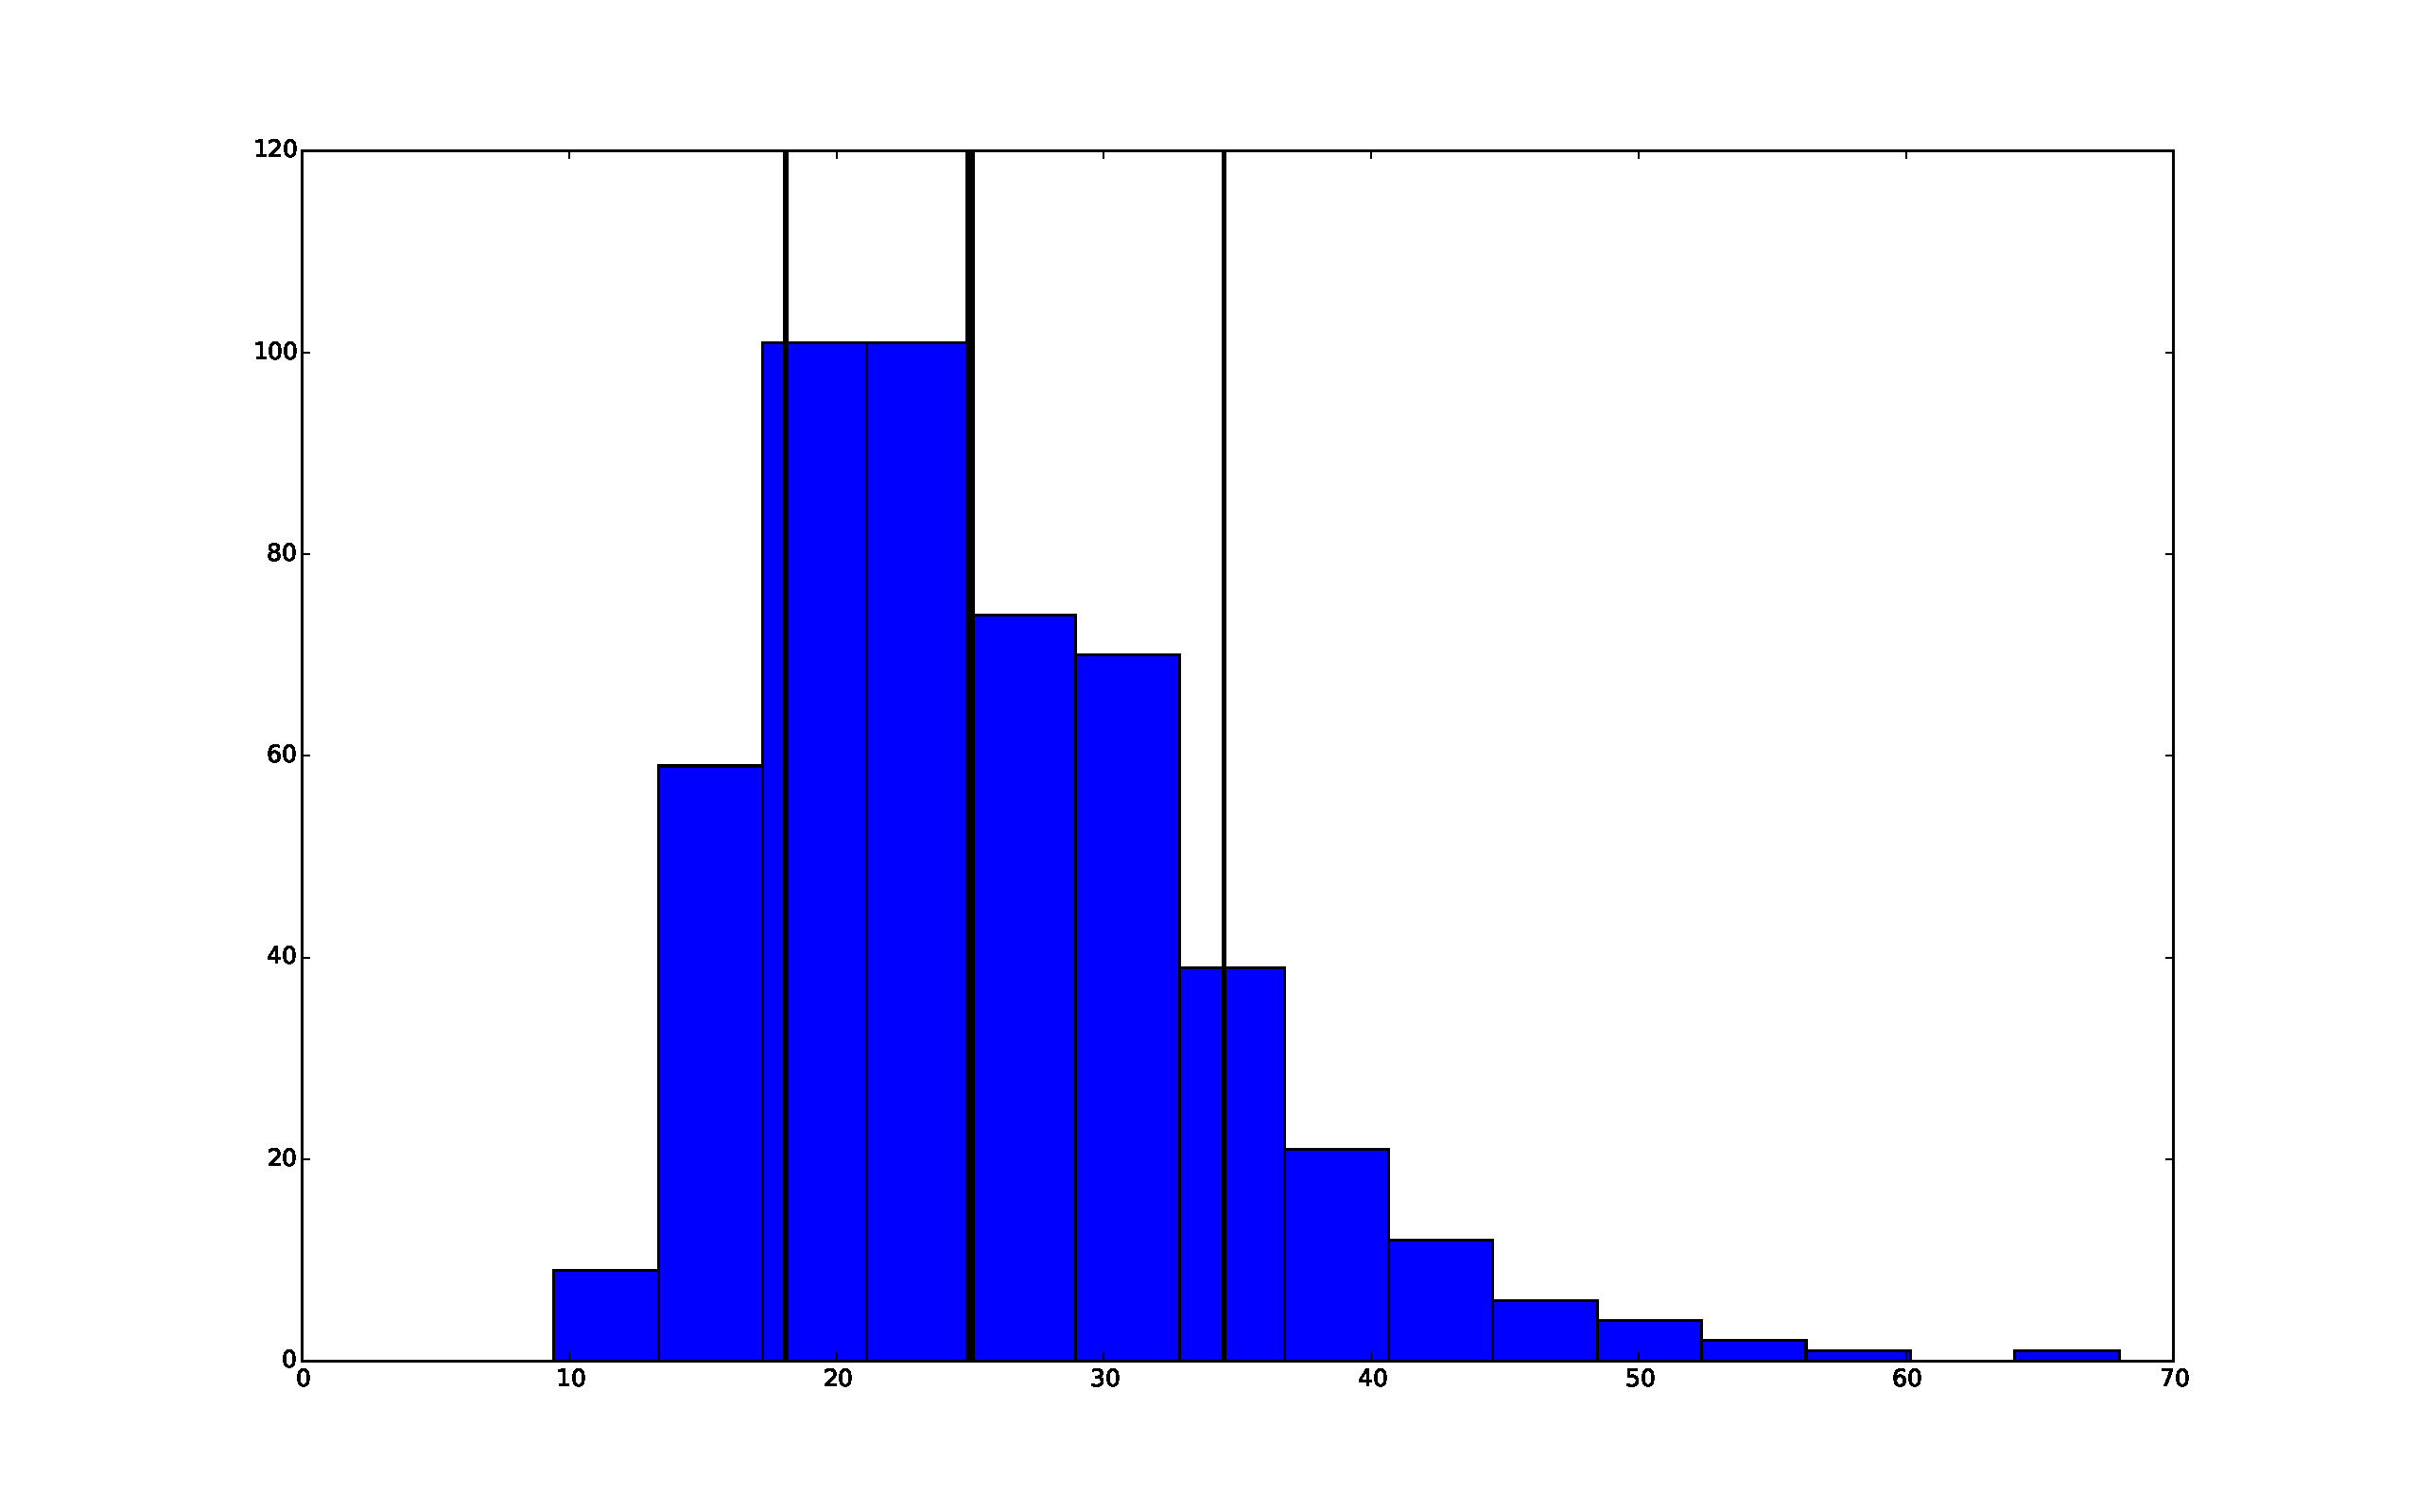
\includegraphics[scale=0.2]{11-23.pdf}
  \end{center}
\caption{\small
Simulated distance measurements to one galaxy!
}
\label{fig:distances}
\end{figure}

\begin{figure}
  \begin{center}
  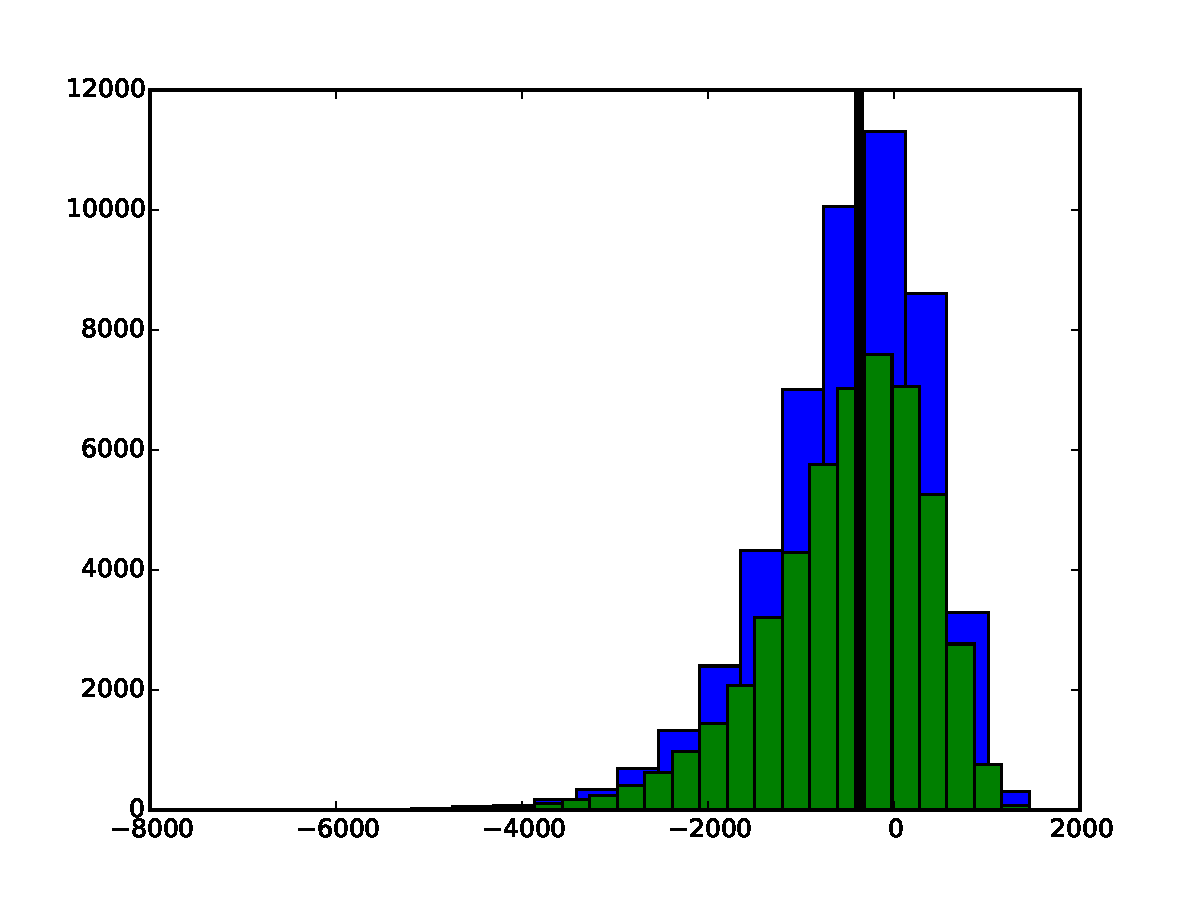
\includegraphics[scale=0.4]{11-23-velocity-normal-est-redo.pdf}
  \end{center}
\caption{\small
The skewed velocity distribution that results from using the normal velocity formula.
}
\label{fig:normalest}
\end{figure}

\begin{figure}
  \begin{center}
  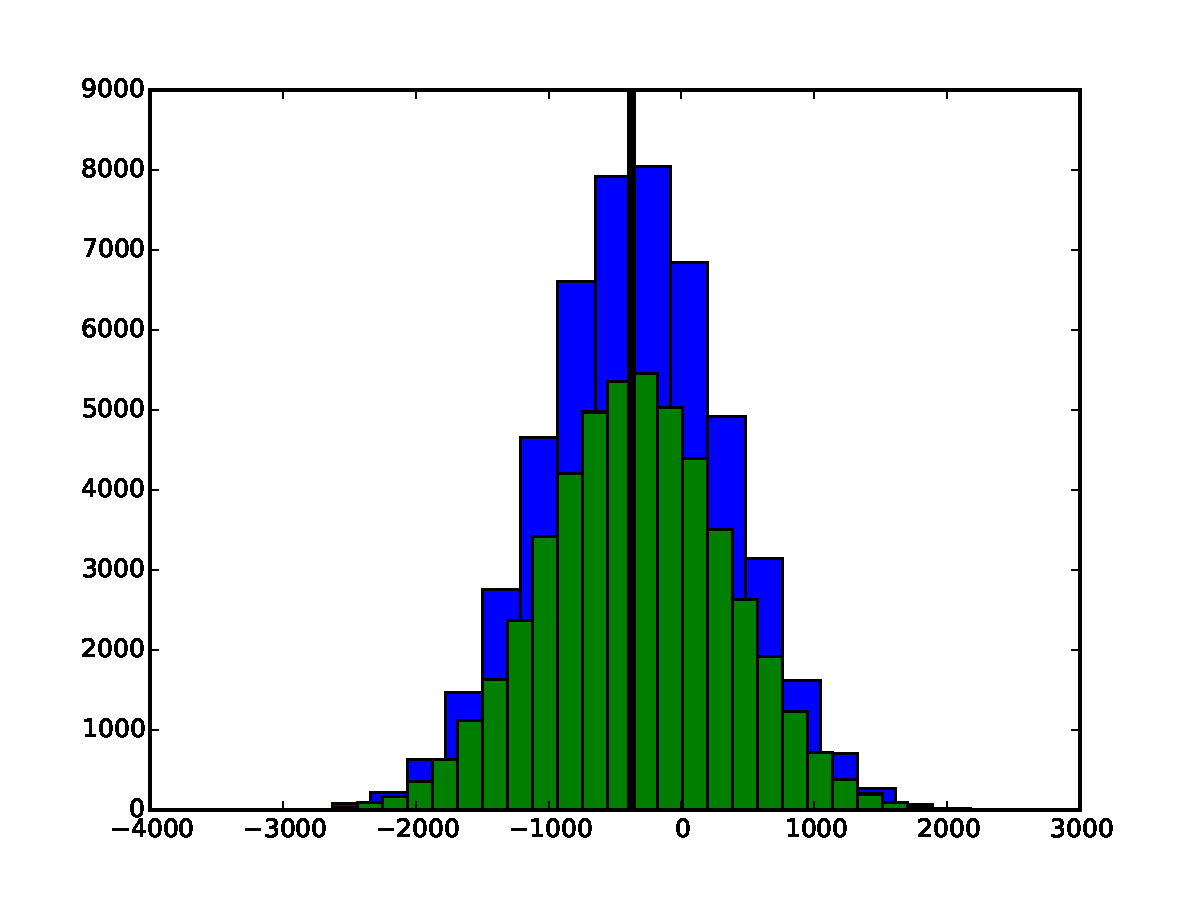
\includegraphics[scale=0.4]{11-23-velocity-feldman-simple-est.pdf}
  \end{center}
\caption{\small
More normal (pun intended) results - obtained by using the new formula.
}
\label{fig:feldmanest}
\end{figure}


\section{Discussion and Conclusions}

Qualitatively, the improved estimator does seem to do a much better job at producing gaussian distributed peculiar velocities. Now that this technique has been tried in Python, it can be easily implemented into the existing logic for many-survey-statistics. Note that this method doesn't work for velocities large compared to redshift, and it also doesn't work for large redshift.

\section{Future work} 
Try out the standard distance modulus formula. Maybe use something like 0.03 error instead of 0.1. The formula Yuyu is using is 
\[
m-M = 5\cdot \log\left(d\right)+25
\]
compared to my formula which is
\[
mod = \ln\left(d\right)
\]
which accounts for the units of d in Mpc, etc.

If possible prove that they're the same with different scaling factors. 
%%%%%%%%%%%%%%%%%%%%%%%%%%%%%%%%%%%%%%%%%%%%%%%%%%%%%%%%%%%%%%%%%%%%%%
%% Finally we specify the format required for our references and the
%% name of the bibtex file where our references should be taken from.
%%%%%%%%%%%%%%%%%%%%%%%%%%%%%%%%%%%%%%%%%%%%%%%%%%%%%%%%%%%%%%%%%%%%%%
\bibliographystyle{mn2e}
\bibliography{paper}
\end{document}

%%%%%%%%%%%%%%%%%%%%%%%%%%%%%%%%%%%%%%%%%%%%%%%%%%%%%%%%%%%%%%%%%%%%%%
%% The end.
%%%%%%%%%%%%%%%%%%%%%%%%%%%%%%%%%%%%%%%%%%%%%%%%%%%%%%%%%%%%%%%%%%%%%%
